%Librerías a usar---------------------------------------------------------------------
\documentclass[11pt, twocolumn]{llncs}
\usepackage[spanish, es-tabla]{babel}
\usepackage[utf8]{inputenc}
\usepackage{amssymb, amsmath}
\usepackage{float}
\usepackage{multicol}
\usepackage{multirow}
\usepackage{geometry}
\usepackage{graphicx}
\usepackage{wrapfig}
\usepackage{listings}
\usepackage{hyperref}
\usepackage{tabularx,booktabs,caption}
\newcolumntype{Z}{>{\raggedright}X}
\renewcommand\spanishtablename{Tabla}
\geometry{top=1in, left=1in, right=1in}

%Inicio del documento-----------------------------------------------------------------
\begin{document}
\twocolumn[

%Título y autores---------------------------------------------------------------------
\title{TIEMPO DE EJECUCIÓN DE UN ALGORITMO DE MULTIPLICACIÓN DE MATRICES CUADRADAS}
\author{
Rodrigo Aguirre  \and 
Germán Contreras \and
Luis Correa \and 
Luciano Grandi  \\ 
 \email{\{rodrigo.aguirrer\}\{german.contrerasa\}\{luis.correac\}\{luciano.grandim\} @utem.cl}
}
\institute{Universidad Tecnológica Metropolitana del Estado de Chile, Santiago, Chile
}
\maketitle 
\begin{@twocolumnfalse}

%Resumen del documento----------------------------------------------------------------
\begin{abstract}
Mediante la implementación de un algoritmo de multiplicación de dos matrices cuadradas, se mostrará la relación entre el tamaño de datos de entrada respecto al tiempo de ejecución del algoritmo en base a un análisis empírico. Con la finalidad de modelar una función que defina la relación existente entre los datos proporcionados, se graficarán los datos para encontrar una ecuación que pueda modelar datos cercanos a los obtenidos, y así, mediante el uso de límites, encontrar el orden de complejidad relacionado al algoritmo.  \\
\\
\textbf{Abstract} By implementing an algorithm for the multiplication of two square matrices, the relationship between the size of the input data with respect to the execution time of the algorithm will be shown based on an empirical analysis. In order to model a function that defines the relationship between the data provided, the data will be plotted to find an equation that can model data close to those obtained, and thus, through the use of bounds, find the order of complexity related to the algorithm. 
\\

%Palabras Clave-----------------------------------------------------------------------
\textit{Palabras Clave:} datos, modelo matemático, algoritmo, tiempos de ejecución, formulación, matrices, ecuación, orden de complejidad, gráfico, optimización, procesamiento, resultados.

\end{abstract}
\end{@twocolumnfalse}
]

%INTRODUCCIÓN------------------------------------------------------------------------
\section{INTRODUCCIÓN}
Las matrices son un tipo de estructura matemática, objeto principal de estudio de la rama del álgebra lineal, relevante en el desarrollo de muchas ciencias. Es utilizada ampliamente para la resolución de sistemas de ecuaciones lineales, derivadas parciales, ecuaciones diferenciales, entre otros; todos estos aplicables a variadas disciplinas como la estadística, economía, física, computación, entre otras.

En las ciencias de la computación, esta estructura es ampliamente utilizada como método de resolución de muchos problemas. Esto se debe a que las matrices son una estructura que agilizan enormemente las operaciones algebraicas, que, utilizando otros métodos, serían tediosos e imprácticos, además de ser una estructura lógica-abstracta fácilmente comprendida por la mente humana, lo que ayuda a la interacción directa con la máquina.

Por ejemplo, las matrices son muy utilizadas en librerías de procesamiento gráfico, debido a su fácil procesamiento vectorial y representación de gráficos tridimensional a bidimensional. 

La informática busca constantemente la optimización de los recursos para la realización de las tareas, principalmente el tiempo y memoria. Debido a que las matrices son una estructura relevante en la mayoría de los procesos informáticos nos es casi imposible no analizar los algoritmos de operación de matrices, sobre todo el de multiplicación, ya que la mayoría de las arquitecturas de procesadores basan sus instrucciones de bajo nivel en sumas y multiplicaciones. 

Utilizando metodologías empíricas, se pretende realizar un experimento de aplicación de un algoritmo de multiplicación de matrices cuadradas, con el fin de analizar el tiempo de ejecución en función del tamaño de datos de entrada n, que en este caso corresponde a la dimensión de las matrices. Con los resultados se espera hallar con el modelo matemático que mejor se ajuste al algoritmo, utilizando técnicas como la regresión lineal. 

Este algoritmo se implementará en lenguaje de programación híbrido C++, reconocido por su alto rendimiento en el manejo de los recursos del sistema. Se aplicará técnicas de programación tradicionales y se utilizará la asignación de memoria dinámica.

Una vez hallado con el modelo matemático se buscará validarlo, realizando un set extra de muestras experimentales que comparen los resultados reales con los obtenidos utilizando el modelo.

A continuación, encontrará una explicación a fondo del propósito, objetivos y metodologías del estudio, así como también el diseño y ejecución del experimento. Usted encontrará un análisis exhaustivo de los resultados obtenidos, así como la conclusión de éste.

%CONTEXTO Y PROPÓSITO DEL EXPERIMENTO------------------------------------------------
\section{CONTEXTO Y PROPÓSITO}\label{contexto_proposito}

Un algoritmo es un conjunto de instrucciones definidas, o secuencias de pasos lógicos que permiten solucionar un problema o realizar una tarea determinada. Estos algoritmos pueden clasificarse acorde a su complejidad, ya sean sencillos o complejos. Al disponer de un algoritmo que funcione correctamente, se nos hace útil determinar ciertos criterios para cuantificar su comportamiento, o en otras palabras, su rendimiento.

Muy seguido se piensa que al hablar de algoritmos sencillos, estos no son competentes. Pero, a la hora de modelar un algoritmo, la sencillez es un componente muy interesante, dado que agiliza el estudio de su eficiencia y su mantenimiento. Cuando hablamos de rendimiento en un algoritmo, este se mide respecto a dos parámetros: el espacio de memoria y el tiempo de ejecución.

Se denomina como tiempo de ejecución de un algoritmo al rango de tiempo t en que un algoritmo comienza su proceso de ejecución hasta el término de este. Este tiempo dependerá de varios factores, tales como la calidad del código o la complejidad del mismo, y los datos de entrada.

Los datos de entrada (dependiendo del tamaño) al interactuar en un algoritmo, tendrán distintos comportamientos y tiempos de ejecución, tal como muchas funciones matemáticas que existen. Esta comparación no es trivial, dado que al saber la complejidad de una función matemática, podemos relacionarla con algún algoritmo y determinar de forma teórica su grado de dificultad. Este grado de dificultad se puede usar para determinar a qué orden de complejidad corresponde cada algoritmo, y así encontrar el que mejor se adapte al problema a solucionar.

Para tal efecto, se desarrollará un algoritmo que pueda crear y multiplicar dos matrices cuadradas de tamaño n. Una matriz es un arreglo bidimensional con un conjunto de datos, ordenados en filas ($i$) y columnas ($j$). Existen diversos tipos de matrices, como las matrices nulas, donde sus datos son solo ceros o las matrices cuadradas como se muestra en la \textit{Fig. 1}, las cuales tienen el mismo número de filas y columnas tal que \textit{n = i = j}.

%PARA PONER IMÁGENES SEGUIR ESTE EJEMPLO
\begin{figure}
\caption{\textit{\label{fig:matrices}Ejemplo de matrices cuadradas}}
\centering
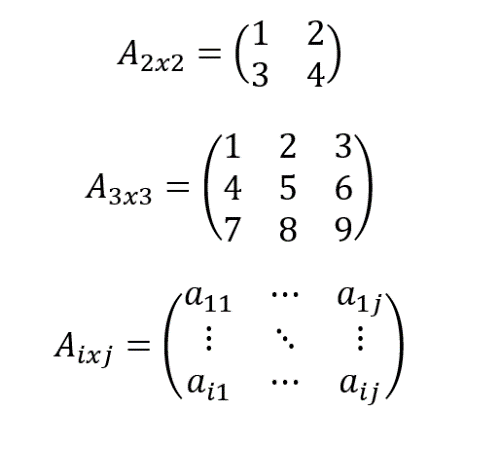
\includegraphics[width=0.3\textwidth]{imagenes/matrices.png}
\end{figure}

El uso de matrices cuadradas no solo está ligado a la programación o al álgebra clásica, sino que también a la economía en operaciones muy complejas como las descomposiciones matriciales de Cholesky y LU. En el ámbito computacional, las matrices son usadas dado su fácil manejo y liviandad para la manipulación de información. Bajo este contexto, son una buena composición para representar diversos tipos de grafos.

La implementación del algoritmo busca formular una función que pueda describir de manera teórica y matemática el comportamiento del tiempo de ejecución en base al tamaño de datos de entrada $n$, por medio de un análisis empírico respecto a la ejecución del algoritmo con distintos valores de entrada de $n$.

Se busca que en base a los valores obtenidos mediante el análisis empírico, estos sean comparados con valores obtenidos en base al modelo matemático formulado, con los mismos valores de entrada $n$ usados anteriormente. Con esto, se espera encontrar un margen de error RDP (\textit{Residual Prediction Deviation}) por cada valor de $n$ usado y explicar los valores RDP que sean interesantes.

El algoritmo en estudio está escrito en lenguaje de programación $C++$. Este algoritmo creará dos matrices cuadradas $A$ y $B$ de tamaño $n$, las cuales estarán pobladas con números enteros positivos aleatorios dentro de un rango definido (desde 1 hasta 100). Con las matrices pobladas, se procederán a multiplicar para formar una nueva matriz cuadrada $C$.

El código del algoritmo es el siguiente:

\lstset{language=, breaklines=true, basicstyle=\footnotesize}
\begin{lstlisting}[frame=single]

#include <iostream>
#include <stdlib.h>
#include <time.h>

using namespace std;

void multmatrix(int n)
{
  int i,j,k;
  long **matriz1=NULL;
  long **matriz2=NULL;
  long **res=NULL;

  matriz1=(long **)malloc(n * sizeof(long *));
  matriz2=(long **)malloc(n * sizeof(long *));
  res=(long **)malloc(n * sizeof(long *));
    
  for (i=0;i<n;i++){
    matriz1[i]=(long *)malloc(n * sizeof(long *));
    matriz2[i]=(long *)malloc(n * sizeof(long *));
    res[i]=(long *)malloc(n * sizeof(long *));
  }
    
  srand(time(NULL));
    
  for(i=0;i<n;i++){
	for(j=0;j<n;j++){
   	  matriz1[i][j]=rand()%100;
      matriz2[i][j]=rand()%100;
    }
  }
  for(i=0;i<n;i++){
    for(j=0;j<n;j++){
      long sum=0;
      for(k=0;k<n;k++){
        sum+=matriz1[j][k]*matriz2[k][i];
      }
      res[j][i]=sum;
    }
  }

  cout<<"Resultado: ";
  for(i=0;i<n;i++){
    for(j=0;j<n;j++){
      cout<<res[i][j];
      cout<<"-";
    }
    cout<<endl;
  }
}

int main(){
  int n;
  cout<<"Valor n: ";
  cin>>n;
  getchar();
  unsigned t0, t1;
  t0=clock();
  multmatrix(n);
  t1=clock();
  double time=(double(t1-t0)/CLOCKS_PER_SEC);
  cout<<"TIEMPO DE EJECUCION: "<<time;
  return 0;
}

\end{lstlisting}

El código diseñado está modelado para recibir valores de entrada de $n$ en un rango aproximado entre 1 a 10000. Para tal efecto, las matrices declaradas tendrán asignación de memoria. Y además, se usa la librería time.h para poder calcular los tiempos de ejecución del algoritmo.

%OBJETIVOS---------------------------------------------------------------------------
\section{OBJETIVOS DEL EXPERIMENTO}\label{objetivos}
Los objetivos son las razones por las cuales se lleva a cabo una acción a corto, mediano o largo plazo. La importancia de los objetivos reside en el hecho de permitir el orden de forma eficiente para saber cómo trabajar o actuar y qué cosas o resultados buscar.

\subsection{Objetivo general}
Medir el tiempo de ejecución de un algoritmo de multiplicación de matrices cuadradas con datos de valores de entrada $n$ y realizar un análisis empírico de los resultados.

\subsection{Objetivos específicos}
\begin{itemize}
    \item Diseñar y ejecutar un experimento a base de un algoritmo.
    \item Recopilar muestras de datos experimentales de la aplicación del algoritmo y analizar los resultados obtenidos en el experimento.
    \item Determinar el modelo matemático en función al tiempo que se ajusta al problema, y así validar el modelo obtenido ejecutando nuevamente el experimento con una serie de datos distintos a los usados anteriormente, para comparar los resultados empíricos con los predichos en el modelo obtenido.
\end{itemize}

%METODOLOGÍA-------------------------------------------------------------
\section{METODOLOGÍA}\label{metodología}
Una buena forma de conseguir resultados esperados, es implementar una metodología que se adapte a las necesidades del estudio, así generando una visión clara y concisa de las acciones relevantes consideradas en la realización del experimento.

\subsection{Reuniones y roles de trabajo}
Para el desarrollo de la actividad, se determinaron sesiones de estudio con una duración de al menos dos horas cada tres días. En cada sesión, se distribuyeron las tareas para cada integrante del equipo, además de planificar las sesiones siguientes.

\subsection{Etapas del experimento}
Para la elaboración del experimento, se eligió un lenguaje de programación fácil de dominar para los integrantes del grupo. Entre las alternativas propuestas por cada integrante (Java, Python, Ruby, C++), se determinó el uso de $C++$ para el desarrollo del algoritmo.

Con el lenguaje elegido, se comenzó a diseñar el algoritmo para multiplicar dos matrices. Cada integrante diseñó un algoritmo respectivo, así escogiendo el más adecuado y eficiente, testeando diversos valores de entrada de $n$ para su correcto funcionamiento.

El diseño del algoritmo se basa en la implementación de dos matrices creadas de forma dinámica dependiendo del valor de entrada de $n$ mediante consola. Para la operación de multiplicación se debe considerar que teniendo dos matrices $A$ y $B$, estas son multiplicables si el número de columnas $i$ de la matriz $A$ es igual que el número de filas $j$ de la matriz $B$. Para la obtención de la matriz producto $C$ se usó la siguiente ecuación matemática:

\begin{equation}
A_{ij} \times B_{jk} = C_{ik}
\end{equation}

En la \textit{Eq. (1)}, el valor del elemento $C_{ik}$ de la matriz producto se obtiene multiplicando cada elemento de la fila $i$ de la matriz $A$ por cada elemento de la columna $j$ de la matriz $B$ y sumándolos. En la \textit{Fig. 2} se muestra el procedimiento de multiplicación de dos matrices pobladas.

\begin{figure}[H]
\caption{\textit{\label{fig:multiplicacion}Proceso de multiplicación de dos matrices}}
\centering
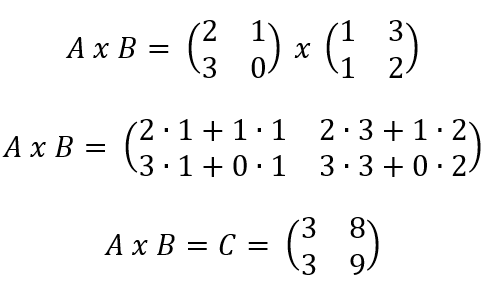
\includegraphics[width=0.4\textwidth]{imagenes/multiplicacion.png}
\end{figure}

Además, se implementó en el código la librería \textit{time.h} para la medición del tiempo de ejecución de la creación de las matrices. Con la librería implementada, se procedió a utilizar la función \textit{clock()}, la cual calcula el tiempo en segundos en el momento que es llamada. A continuación se muestra el código para el cálculo del tiempo de ejecución:

\lstset{language=, breaklines=true, basicstyle=\footnotesize}
\begin{lstlisting}[frame=single]

//Funcion multiplicacion de matrices
void multmatrix(int n){
...
}

//Funcion principal
int main(){
  ...
  //Creacion de variables enteras sin signo
  unsigned t0, t1;
  
  //Llamada de la funcion clock() para el comienzo del tiempo del algoritmo
  t0=clock();
  
  //Llamada de la funcion multiplicacion
  multmatrix(n);
  
  //Llamada de la funcion clock() para el termino del tiempo del algoritmo
  t1=clock();
  
  //Creacion de variable con el tiempo final de ejecucion del algoritmo
  double time=(double(t1-t0)/CLOCKS_PER_SEC);
  ...
}

\end{lstlisting}

Todo el código implementado para la elaboración del experimento está en la sección 2 de este documento (CONTEXTO Y PROPÓSITO).

Cada tiempo de ejecución entregado por el código fue recolectado y tabulado, con el fin de generar un gráfico en las coordenadas $x$ e $y$ en el plano cartesiano obteniendo su regresión adecuada y respectiva formulación del modelo matemático.

\subsection{Herramientas de hardware}
Se ha usado para el experimento un computador portátil con las siguientes características:

\begin{itemize}
    \item $CPU$: AMD Ryzen 3 2200U con Radeon Vega Mobile 2,5 GHz quadcore.
    \item $RAM$: 8 GB (1 x 8 GB) DDR4 a 2400 mhz SODIMM.
    \item $Memoria$: x 1 Unidad SSD NVME Western Digital de 250 GB.
\end{itemize}

\subsection{Herramientas de software}
Para el desarrollo del experimento se ha usado el sistema operativo Windows 10 Pro x64, el lenguaje de programación $C++$, junto con el entorno de desarrollo \textit{Code::Blocks V22.04 x64} y con el compilador \textit{ggc compiler} integrado. Para la tabulación y regresión del modelo matemático se ha usado el programa \textit{Microsoft Excel}. Para el diseño de gráficos de funciones se ha utilizado $Geogebra$, un software matemático online.

Además, se usara como complemento el sistema operativo \textit{Manjaro x64 Kernell Linux 5.9.10-1}, esto con el fin de tener la claridad si el uso de diferentes sistemas operativos pudiera llegar a afectar en el rendimiento de un mismo algoritmo.

%DISEÑO DEL EXPERIMENTO-------------------------------------------------------------
\section{DISEÑO DEL EXPERIMENTO}\label{diseño}
En el presente experimento se mantendrán constantes las herramientas de hardware y software, esto con el fin de que no se vean afectados los resultados en las diferentes mediciones. Sin embargo, se realizarán mediciones extras en diferentes condiciones de hardware y software, con el fin de obtener nuevos datos para una posible conclusión con respecto a las variaciones que podría llegar a tener el experimento si se varía en la elección de hardware y software.

Para realizar las mediciones en un hardware y software diferente se usará un computador de escritorio con las siguientes características:

\begin{itemize}
    \item $CPU$: Intel Core™ i7-8700 Caché de 12 M, hasta 4,60 GHz.
    \item $Ram$: 16 GB (2 x 8 GB Dual Channel) DDR4 a 2666 mhz.
    \item $Memoria$:
        \begin{itemize}
             \item x 1 Unidad SSD Kingston SSDNow A400 240GB
        	 \item x 1 Unidad SSD 1TB Kingston A2000, M.2 2280, NVMe
        	 \item x 1 Disco Duro 1TB WD Blue 3.5
        \end{itemize}
    \item \textit{Sistema Operativo}: Windows 10 Pro x64.
\end{itemize}

Pasando al experimento, se usarán diferentes valores de $n$ para realizar la medición, siendo el valor mínimo posible para poder realizar la medición $2$ y como valor máximo no se estableció un número debido a que teóricamente se podría llegar a calcular cualquier valor, sin embargo, el aumento en tiempo a medida que se aumenta n es exponencial, y es por esta misma situación que para el experimento se estableció que el valor máximo a calcular por el grupo de trabajo será de $2000$, abriéndose a la posibilidad de que si las herramientas de hardware lo permiten, poder calcular valores más grandes de $n$ para mejorar la precisión del experimento.

Con el fin de que cada una de las mediciones tenga una precisión mas exacta y que se pueda llegar a resultados más concluyentes, es que se definió que para cada valor de $n$ se realizarán tres mediciones, ya que el sólo tomar en cuenta una medición podría llegar a afectar el experimento, esto debido, a que como se menciona anteriormente el hardware influye en los resultados del experimento, y si este por algún motivo se ve afectado durante el experimento, el valor obtenido podría llegar a no ser concluyente, y para asegurar que estos resultados no se vean afectados, es que el grupo de trabajo tomará éstas mediciones para un mismo valor de $n$ en horarios diferentes del día.

Luego de obtener los resultados, es que mediante el programa Excel se agregarán todos los datos obtenidos a una tabla, y su respectivo $n$ para así poder generar un gráfico que permita calcular la precisión de estos datos y la fórmula teórica que nos ayudaría a saber cuanto tiempo es que se podrían llegar a demorar mediciones futuras.

Los datos obtenidos junto con su gráfico, serán analizados por el grupo de trabajo, y se realizará una comparación en la que se calcule mediante la fórmula obtenida el resultado teórico y posteriormente, una comparación con el dato obtenido realmente. Esto con el fin de asegurar la calidad del experimento y saber si es que los datos finalmente fueron concluyentes o la medición se vio afectada por diversos motivos.

%EJECUCIÓN DEL EXPERIMENTO-------------------------------------------------------------
\section{EJECUCIÓN DEL EXPERIMENTO}\label{ejecucion}
El tiempo que tomó realizar este experimento
fue de aproximadamente unas tres horas,
ya que se tomaron un total de 117 mediciones para 13 valores de n. Esto debido a que se realizaron las pruebas en distintos sistemas operativos dentro de la misma máquina y en otra máquina con uno de los sistemas operativos utilizados y distinto hardware.

No se presentaron problemas en la ejecución del experimento, pero si una diferencia notable en la ejecución del algoritmo.

%RESULTADOS OBTENIDOS-------------------------------------------------------------
\section{RESULTADOS OBTENIDOS}\label{resultados}
Con los valores obtenidos, se elaboró la siguiente tabla:

\begin{table}[H]
\caption{\textit{Tiempos de ejecución del algoritmo respecto a \textbf{n} con Windows y Linux}}\label{tab:tabla1}
\begin{tabularx}{\columnwidth}{ | >{\centering\arraybackslash}X | >{\centering\arraybackslash}X | >{\centering\arraybackslash}X |} \hline
$n$ & T[s] prom. ($Windows$) & T[s] prom. ($Linux$)  \\ \hline
2 & 0,000 & 4,3x$10^{-5}$ \\
5 & 0,015 & 9,9x$10^{-5}$ \\
10 & 0,015 & 1,1x$10^{-4}$ \\
20 & 0,057 & 2,7x$10^{-4}$ \\
50 & 0,339 & 0,002 \\
100 & 1,432 & 0,044 \\
200 & 5,718 & 0,049 \\ 
250 & 8,608 & 0,084 \\ 
500 & 33,516 & 0,513 \\ 
750 & 64,917 & 1,724 \\
1000 & 128,803 & 3,833 \\ 
1500 & 257,952 & 14,082 \\ 
2000 & 514,581 & 38,143 \\ \hline
\end{tabularx}
\end{table}

En la \textit{Fig. 3} se muestra el gráfico el tiempo de ejecución del algoritmo respecto a los valores de entrada de $n$ en el sistema operativo Windows 10 Pro x64 en función de los datos de la \textit{Tabla 1}:

\begin{figure}[H]
\caption{\textit{\label{fig:grafico1}Gráfico de Tiempo de ejecución respecto a valores de entrada de \textbf{n} en Windows 10}}
\centering
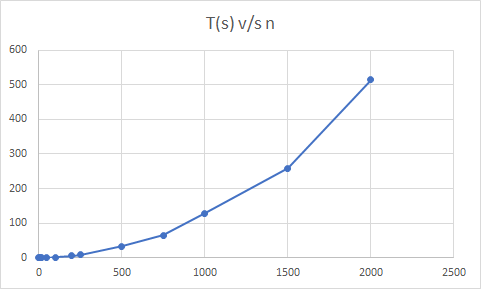
\includegraphics[width=0.47\textwidth]{imagenes/grafico_1.png}
\end{figure}

En la \textit{Fig. 4} se muestra el gráfico el tiempo de ejecución del algoritmo respecto a los valores de entrada de $n$ en el sistema operativo Manjaro x64 Kernell Linux 5.9.10-1:

\begin{figure}[H]
\caption{\textit{\label{fig:grafico2}Gráfico de Tiempo de ejecución respecto a valores de entrada de \textbf{n} en el sistema operativo Linux Manjaro}}
\centering
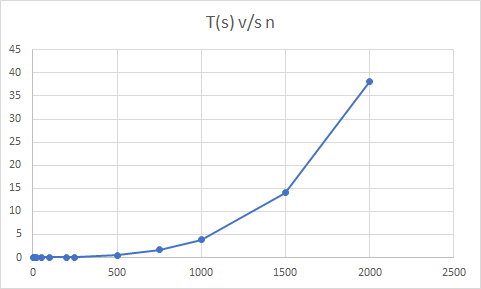
\includegraphics[width=0.47\textwidth]{imagenes/grafico_2.png}
\end{figure}

A continuación se muestra la tabla de datos con los valores obtenidos del algoritmo ejecutado en un computador de escritorio con hardware distinto al usado, como se mencionó en la sección 5 de este documento (DISEÑO DEL EXPERIMENTO):

\begin{table}[H]
\caption{\textit{Tiempos de ejecución del algoritmo respecto a \textbf{n} con distinto hardware}}\label{tab:tabla2}
\begin{tabularx}{\columnwidth}{ | >{\centering\arraybackslash}X | >{\centering\arraybackslash}X | >{\centering\arraybackslash}X |} \hline
$n$ & T[s] prom. ($Windows$) \\ \hline
2 & 0,001 \\
5 & 0,004 \\
10 & 0,017 \\
20 & 0,070 \\
50 & 2,062 \\
100 & 3,127 \\
200 & 9,027 \\ 
250 & 13,137 \\ 
500 & 42,907 \\ 
750 & 93,611 \\
1000 & 172,328 \\ 
1500 & 397,900 \\ 
2000 & 704,870 \\ \hline
\end{tabularx}
\end{table}

En la \textit{Fig. 5} se muestra el gráfico el tiempo de ejecución del algoritmo respecto a los valores de entrada de $n$ con el hardware distinto usado en función de los datos de la \textit{Tabla 2}:

\begin{figure}[H]
\caption{\textit{\label{fig:grafico3}Gráfico de Tiempo de ejecución respecto a valores de entrada de \textbf{n} con hardware distinto al usado anteriormente}}
\centering
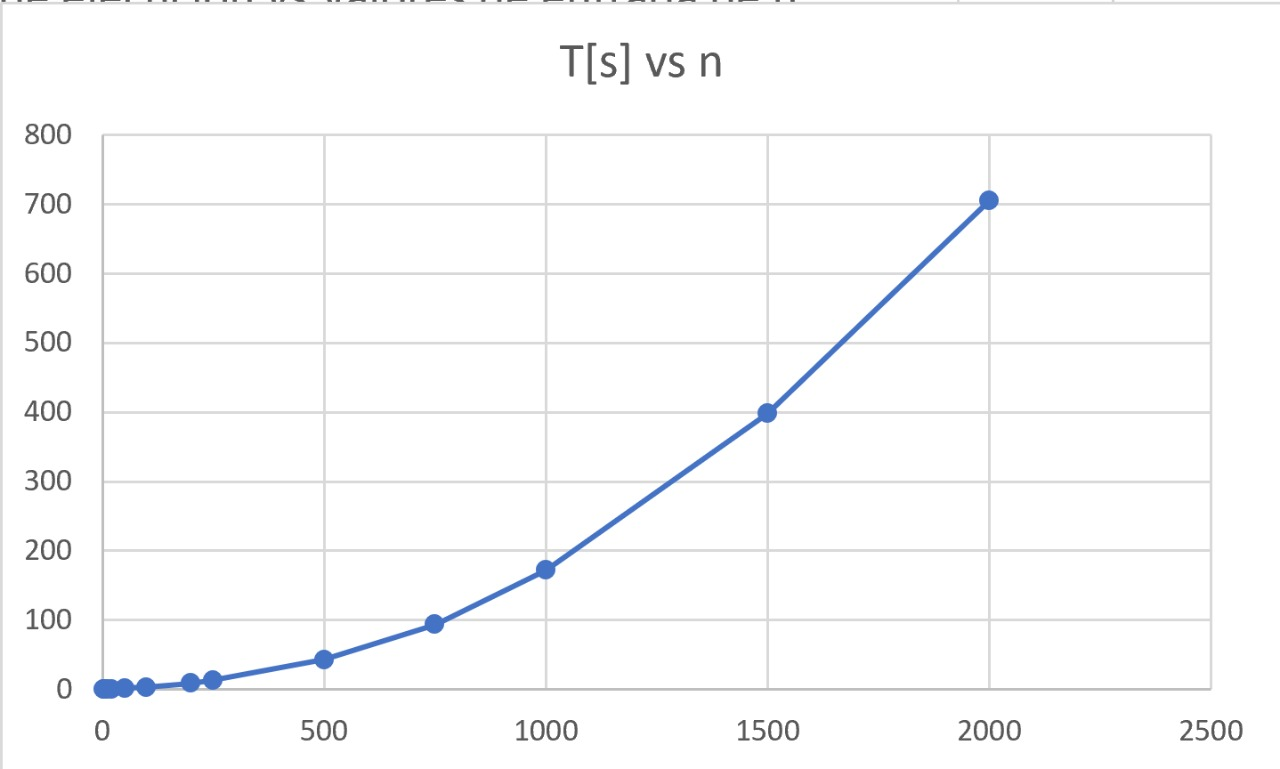
\includegraphics[width=0.47\textwidth]{imagenes/grafico_3.jpeg}
\end{figure}

%ANÁLISIS DE RESULTADOS-------------------------------------------------------------
\section{ANÁLISIS DE RESULTADOS}\label{analisis}
Para realizar el análisis del experimento, se decidieron utilizar los datos de los tiempos de ejecución del algoritmo en el sistema operativo Manjaro x64 Kernell Linux 5.9.10-1. Esta decisión se debe a que las muestras obtenidas fueron más estables y presentaron un mejor rendimiento con respecto a lo que se obtuvo en Windows 10 Pro x64 (tomando en consideración el mismo hardware en ambos sistemas operativos).

En la \textit{Tabla 3} se muestran los datos obtenidos con la ejecución del algoritmo desde el sistema operativo Manjaro x64 Kernell Linux 5.9.10-1.

\begin{table}[H]
\caption{\textit{Tiempos de ejecución del algoritmo respecto a \textbf{n} en Manjaro Linux}}\label{tab:tabla3}
\begin{tabularx}{\columnwidth}{ | >{\centering\arraybackslash}X | >{\centering\arraybackslash}X |} \hline
$n$ & T[s] prom. ($Linux$)  \\ \hline
2 & 4,3x$10^{-5}$ \\
5 & 9,9x$10^{-5}$ \\
10 & 1,1x$10^{-4}$ \\
20 & 2,7x$10^{-4}$ \\
50 & 0,002 \\
100 & 0,044 \\
200 & 0,049 \\ 
250 & 0,084 \\ 
500 & 0,513 \\ 
750 & 1,724 \\
1000 & 3,833 \\ 
1500 & 14,082 \\ 
2000 & 38,143 \\ \hline
\end{tabularx}
\end{table}

Utilizando los datos de la \textit{Tabla 3} se realizó un gráfico de tiempo de ejecución respecto a la entrada de datos, donde la entrada de datos es la variable independiente y el tiempo de ejecución la variable dependiente. Hecho esto, usando el software de hojas de cálculo Microsoft Excel se utilizó la herramienta de línea de tendencia para realizar una regresión lineal, ergo, determinar el modelo matemático que mejor se ajusta al comportamiento temporal del algoritmo en estudio, considerando si $R^2$ se acerca a $1$ para escoger la más adecuada.

\begin{figure}[H]
\caption{\textit{\label{fig:grafico4}Modelo obtenido mediante regresión lineal sobre los tiempos de ejecución del algoritmo en sistema operativo Manjaro Linux}}
\centering
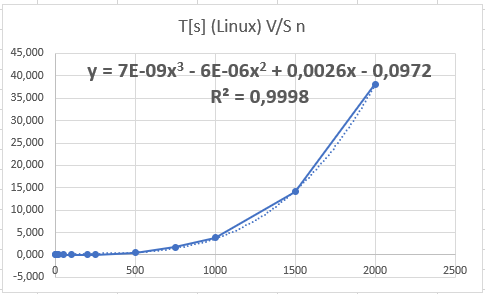
\includegraphics[width=0.47\textwidth]{imagenes/grafico_4.png}
\end{figure}

Como se puede apreciar en la \textit{Fig. 6}, La regresión lineal aplicada sobre los puntos del gráfico muestra un modelo matemático de tendencia polinómica de grado 3, con un error $R^{2}$ = 0,9998. La ecuación obtenida queda de la siguiente forma:

{
\scriptsize
\begin{equation}
{T(n)=(7 \cdot 10^{-9})n^3-(6 \cdot 10^{-6})n^2+0,0026n-0,0972}
\end{equation}
}

Con la \textit{Eq. (2)} elaborada, se procede a determinar el comportamiento en el peor de los casos de esta ecuación mediante análisis teórico. Para ello, se debe buscar un valor $n_0$ mayor que cero y un valor $c$ mayor que cero, tal que se cumpla lo siguiente:

\begin{equation}
T(n) \leq f(n), \forall n_0
\end{equation}

Donde en la \textit{Eq. 3}, $f(n)$ es una función de cota superior para explicar el comportamiento de $T(n)$, siempre y cuando el argumento sea infinito.

La \textit{Eq. (2)} al ser polinómica de grado 3, definiremos $f(n)$ = $n^3$, con valores de $c$ = 2,7x$10^{-4}$ y $n_{0}$ = 20, tal que podamos obtener una expresión como la siguiente:

\begin{equation}
T(n_{0}) \leq cf(n_{0}).
\end{equation}

Al calcular $T(n_{0})$ con $n_{0}$ = 20 nos da un resultado de
-0,047, y en $cf(n_{0})$ = 2,16, de forma que se cumple la \textit{Eq. (4)}. Por tanto, los valores de $c$ y $n_0$ son completamente válidos.

Para estudiar el comportamiento que tendrá $T(n)$ en el peor de los casos cuando $n$ $\longrightarrow$ $\infty$, se aplicará un análisis asintótico en la \textit{Eq. (4)} usando la teoría de límites como se muestra en la \textit{Eq. (5)} y \textit{Eq. (6)}:

\begin{equation}
\lim_{n\rightarrow\infty}(T(n_{0})) \leq \lim_{n\rightarrow\infty}(cf(n_{0}))
\end{equation}

\begin{equation}
\lim_{n\rightarrow\infty}(-0,047) \leq \lim_{n\rightarrow\infty}(2,16)
\end{equation}

Resolviendo la \textit{Eq. (5)} nos da un resultado de -0,047 $\leq$ 2,16. Por tanto, podemos concluir que el comportamiento de nuestra ecuación $T(n)$, si es menor o igual que la función $cf(n)$ cuando $T(n)$ $\rightarrow$ $\infty$ con $f(n)$ = $n^{3}$ tiene un \textit{Orden de Complejidad} de $O(n^{3})$, para todos los valores de $n$ mayores o igual a 20.

\subsection{Validación del modelo}

Para comprobar si la ecuación entrega valores estimativos y/o referenciales de tiempo de ejecución con respecto a los obtenidos mediante la aplicación del algoritmo, se han anotado los errores porcentuales (RDP) correspondientes en la \textit{Tabla 4}, así mostrando el sesgo de cada valor declarado por $n$.

\begin{table}[H]
\caption{\textit{Tiempos de ejecución del algoritmo respecto a \textbf{n} en comparación con los datos obtenidos de forma experimental y mediante fórmula junto con su error porcentual}}\label{tab:tabla4}
\begin{tabularx}{\columnwidth}{ | >{\centering\arraybackslash}X | >{\centering\arraybackslash}X | >{\centering\arraybackslash}X | >{\centering\arraybackslash}X |} \hline
$n$ & T[s] prom. & T(n)[s] & RDP\\ \hline
2 & 0,001 & $\Delta$-0,092 & 101\% \\
5 & 0,001 & $\Delta$-0,084 & 101\% \\
10 & 0,001 & $\Delta$-0,071 & 100\% \\
20 & 0,001 & $\Delta$-0,047 & 100\% \\
50 & 0,002 & $\Delta$0,019 & 89.47\% \\
100 & 0,044 & $\Delta$0,109 & 59,633\% \\
200 & 0,049 & $\Delta$0,239 & 79,498\% \\ 
250 & 0,084 & $\Delta$0,287 & 70,732\% \\ 
500 & 0,513 & $\Delta$0,578 & 11,246\% \\ 
750 & 1,724 & $\Delta$1,431 & 20,475\% \\
1000 & 3,833 & $\Delta$3,503 & 9,421\% \\ 
1500 & 14,082 & $\Delta$13,928 & 1,106\% \\ 
2000 & 38,143 & $\Delta$37,103 & 2,726\% \\ \hline
\end{tabularx}
\end{table}


\subsection{Predicciones con el modelo}
En la \textit{Tabla 5} se mostrará algunos valores de entrada de $n$ que pueden resultar interesantes de observar, tanto en comportamiento del dato, como del tiempo de ejecución.

\begin{table}[H]
\caption{\textit{Tiempos de ejecución del algoritmo respecto a \textbf{n} en comparación a los datos obtenidos con la ecuación resultante del modelo matemático formulado.}}\label{tab:tabla5}
\begin{tabularx}{\columnwidth}{ | >{\centering\arraybackslash}X | >{\centering\arraybackslash}X | >{\centering\arraybackslash}X |} \hline
$n$ & T(n)[s] ($Linux$) \\ \hline
1250 & $\Delta$7,449 \\
1750 & $\Delta$23,593 \\
2150 & $\Delta$47,326 \\
5000 & $\Delta$737,903 \\
7000 & $\Delta$2.125,100 \\
10000 & $\Delta$6.425,900 \\
20000 & $\Delta$5.3651,900 \\ 
50000 & $\Delta$86.0130,000 \\ 
100000 & $\Delta$6.940.260,000 \\ 
1000000 & $\Delta$6.994.002.599,900 \\
 \hline
\end{tabularx}
\end{table}

Con estos resultados se puede  verificar que en base a la ecuación obtenida en la validación del modelo es posible estimar tiempos de ejecución con respecto a valores de $n$.
%CONCLUSIONES-------------------------------------------------------------
\section{CONCLUSIONES}\label{conclusiones}

De acuerdo a lo mostrado anteriormente, se puede demostrar que los objetivos propuestos se cumplieron satisfactoriamente, y en base a esto es que se puede llegar a varias conclusiones.

Luego de calcular todos los datos requeridos y analizarlos, se puede ver que los tiempos responden a una función polinómica de carácter exponencial por lo que a medida que se aumente la variable de entrada $n$, el tiempo requerido para poder llegar al resultado, irá en ascenso con una gran diferencia respecto al anterior.

El algoritmo utilizado, de acuerdo a los datos obtenidos, varía demasiado en el tiempo que se demora en realizar el cálculo de la multiplicación de dos matrices con diferentes hardware y diferentes sistemas operativos. Pudiendo llegar a notar un gran aumento en el tiempo de hasta un 1350\% aproximadamente.

Con respecto a los valores de RDP, si bien se ve que estos pueden llegar a superar el 100\% de diferencia, esto es solamente porque los tiempos calculados son demasiado pequeños, y posteriormente se demuestra que el modelo se valida, ya que los valores de RDP fueron bajando en cálculos que llegaban a tiempos más grandes, en los que la diferencia era mínima, llegando incluso a un valor de RDP de 1,1\% aproximadamente.

Luego de realizar todas las mediciones mostradas, se llegó a la conclusión de que la mejor combinación de hardware y software, es en el computador portátil con el procesador AMD Ryzen 3 2200U con Radeon Vega Mobile 2,5 GHz quadcore y el sistema operativo Manjaro x64 Kernell Linux 5.9.10-1. Si bien no se pudo llegar a una respuesta clara del por qué el cálculo del número fue mas rápido en un procesador de menor gama. La información recopilada en conversaciones con académicos, nos ayudó a entender que ésto se podría deber al ALU que tiene el procesador, pero al buscar información sobre esto con el modelo especifico no se pudo encontrar.

%------------------------------------------------------------------------

\end{document}